% ------------------------------------------------------------
\section{Calendar Week}
% ------------------------------------------------------------
% --------------------------------------------------- Slide --
\subsection{CW 26}
% ------------------------------------------------------------
\begin{frame}
  \frametitle{Review CW 26}
	\begin{itemize}
		\item "Anerkennung" -> Provide documentation for KMK verification - \textcolor{green}{Done} 
		\item First simplified analytical model (simple cantilever beam for titanium implant) run with Kitamura2004 dimensions, material properties, loads, etc.
	\end{itemize}
\end{frame}

\begin{frame}
  \frametitle{Review CW 26 - First Model}
	\begin{figure}
		%\centering
		\subfigure{
		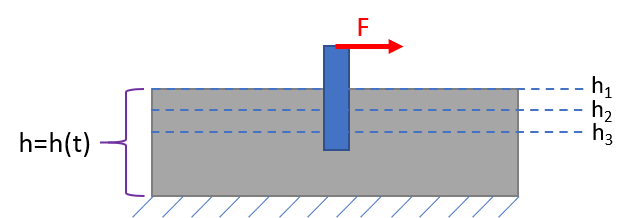
\includegraphics[width=0.45\textwidth]{pictures/CW26_1}
		}
		%\quad
		\subfigure{
		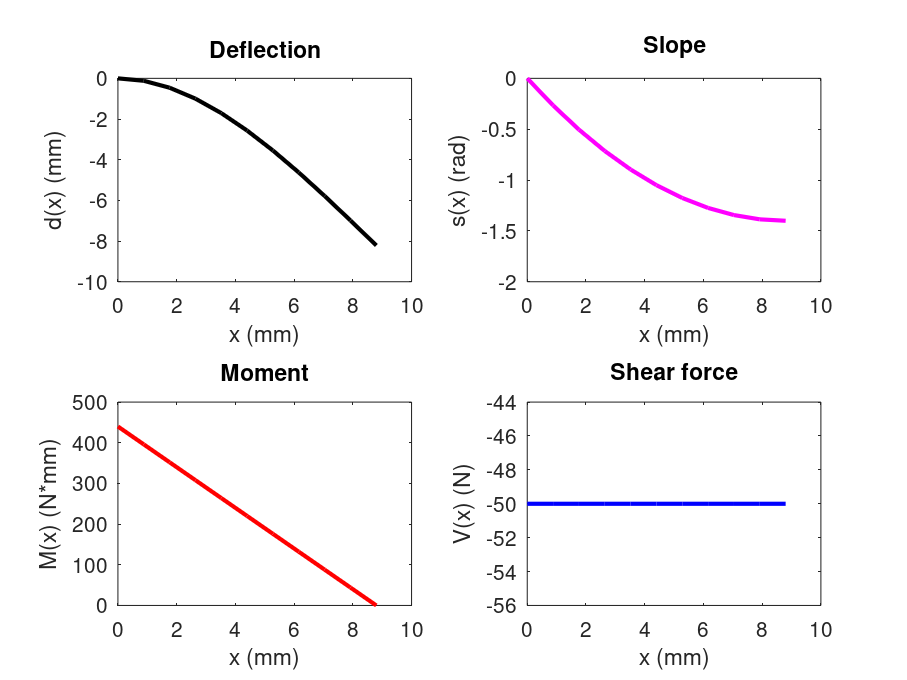
\includegraphics[width=0.45\textwidth]{pictures/CW26_2}
		}
	\end{figure}
\end{frame}
% ------------------------------------------------------------
% --------------------------------------------------- Slide --
\subsection{CW 27+28}
% ------------------------------------------------------------
% ------------------------------------------------------------
\begin{frame}
  \frametitle{Outlook CW 27 + 28}
	\begin{itemize}
		\item Vacation in CW 27. No work planned. No update will be sent.
		\item Presence at MHH in CW 28 (Tuesday, 13th July). Plan:
		\begin{itemize}
			\item Use Ansys at MHH PC to compare stress results from simplified approach with FEA model created at last visit.
			\item Visit to library.
			\item Eventually clarify any formalities .
		\end{itemize}
	\end{itemize}
\end{frame}
% --------------------------------------------------- Slide --

